\documentclass[13pt]{article}
\usepackage{amsmath, amsthm, amssymb, graphicx, enumitem, esvect}


% Language setting
% Replace `english' with e.g. `spanish' to change the document language
\usepackage[english]{babel}

% Set page size and margins
% Replace `letterpaper' with `a4paper' for UK/EU standard size
\usepackage[letterpaper,top=2cm,bottom=2cm,left=3cm,right=3cm,marginparwidth=1.75cm]{geometry}

\title{C\&EE 110 Homework 1}
\author{Warren Kim}

\begin{document}
\maketitle

\newpage
\section*{Problem 1}
\begin{enumerate}[label=\alph*)]
\item Using Sturge's rule, compute the proper number of intervals for this data sample.
\item Using the number of bins from part a), report the histogram for this data sample.
\item Compute the sample mean and sample standard deviation.
\end{enumerate}

\subsection*{Response}
\begin{enumerate}[label=\alph*)]
\item $k = \lfloor 1 + 3.3log_{10}(n) \rfloor = \lfloor log_{10}(1 + 3.3(100)) \rfloor = 7$

\item The histogram has $k = 7$ bins and a bin width of $\frac{max - min}{bins} = \frac{10.31 - 1.11}{7} = 1.314$ \\
  \begin{center}
    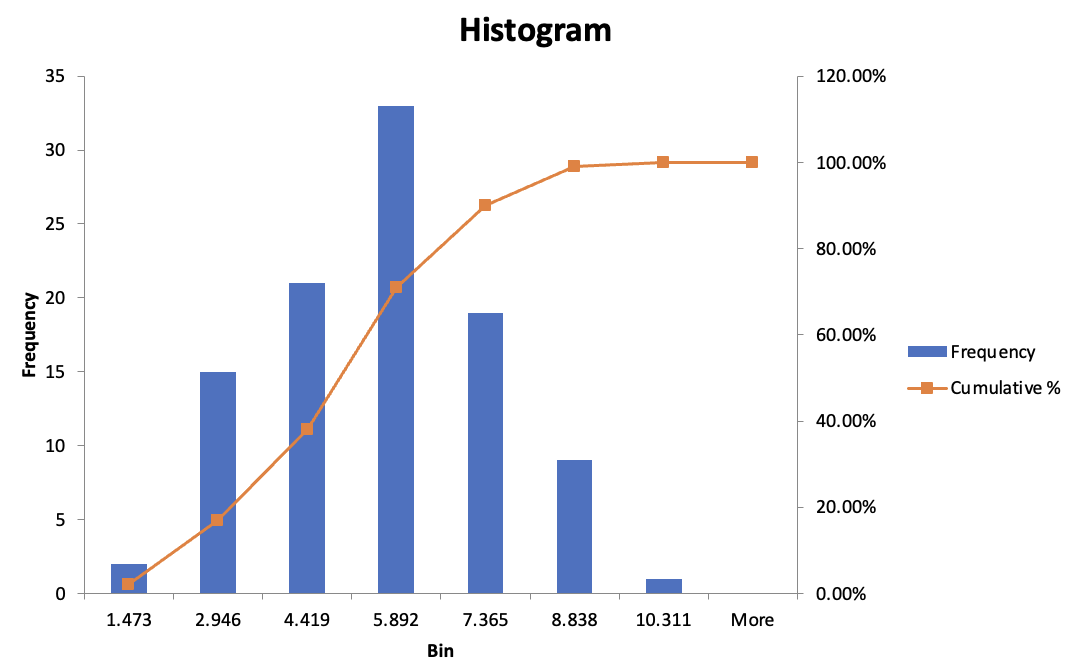
\includegraphics[scale=0.6]{figures/histogram.png}    
  \end{center}

\item The formula for sample mean $\overline{y}$ and sample standard deviation $s$ are:
  \[\overline{y} = \frac{\sum_{i = 1}^{n} y_i}{n}\]
  \[s = \sqrt{\frac{\sum_{i = 1}^{n} (y_i - \overline{y})^2}{n - 1}}\]
  Sample mean:
  \begin{align*}
    \overline{y} &= \frac{\sum_{i = 1}^{n} y_i}{n} \\
                 &= \frac{\sum_{i = 1}^{100}y_i}{100} \\
    \overline{y} &= 4.888
  \end{align*}
  Sample standard deviation:
  \begin{align*}
    s &= \sqrt{\frac{\sum_{i = 1}^{n} (y_i - \overline{y})^2}{n - 1}} \\
      &= \sqrt{\frac{\sum_{i = 1}^{100} (y_i - 4.889)^2}{100 - 1}} \\
    s &= 1.884
  \end{align*}
\end{enumerate}

\newpage
\section*{Problem 2}
The time taken by college-age students to complete an obstacle course is approximately
normally distributed with a mean of 45 seconds and a standard deviation of 7.2 seconds.
What fraction of all students finished the obstacle course in the following intervals?
\begin{enumerate}[label=\alph*)]
\item 37.8 to 52.2 seconds
\item More than 30.6 and less than 66.6 seconds
\item Less than 59.4 seconds
\item Less than 23.4 or more than 66.6 seconds
\item What is the largest standard deviation acceptable to assume the data is normally distributed?
  (Hint: the time should always be positive or equal to zero.)
\end{enumerate}

\subsection*{Response}
Let $\overline{y} = 45,\ s = 7.2$ be the sample mean and standard deviation respectively.
\begin{enumerate}[label=\alph*)]
\item $37.8 = \overline{y} - s, \ 52.2 = \overline{y} + s$. By the empirical rule, the interval captures $68\%$.
\item $30.6 = \overline{y} - 2s, \ 66.6 = \overline{y} + 3s$. By the empirical rule, the interval captures
  $47.5\% + 49.85\% = 97.35\%$.
\item $59.4 = \overline{y} - 2s$. By the empirical rule, the interval captures $\frac{95}{2}\% + 50\% = 97.5\%$.
\item $23.4 = \overline{y} - 3s, \ 66.6 = \overline{y} + 3s$. By the empiricle rule, the interval captures
  $100\% - 99.7\% = 0.3\%$.
\item
  \begin{align*}
    45 - 3s &= 0 \\
    3s &= 45 \\
    s &= 15
  \end{align*}
  The largest standard deviation acceptable to assume the data is normally distributed is $15$ seconds.
\end{enumerate}

\newpage
\section*{Problem 3}
Show that
\[\sum_{i = 1}^{n} (y_i - \overline{y})^2 = \sum_{i = 1}^{n} y_i^2 - \frac{1}{n} \bigg(\sum_{i = 1}^{n} y_i\bigg)^2\]
And calculate the sample variance $s^2$ based on the following information:
\[\sum_{i = 1}^{n} y_i^2 = 40, \ \sum_{i = 1}^{n} y_i = 14, \ n = 6\]
Hint:
\begin{align*}
  \sum_{i = 1}^{n} (x_i \pm y_i) &= \sum_{i = 1}^{n} x_i \pm \sum_{i = 1}^{n} y_i && (1) \\
  \sum_{i = 1}^{n} cy_i &= c \sum_{i = 1}^{n} y_i && (2) \\
  \sum_{i = 1}^{n} c &= nc && (3) \\
  \sum_{i = 1}^{n} y_i &= n\overline{y} && (4)
\end{align*}
\subsection*{Response}
\begin{proof}
  \begin{align*}
    \sum_{i = 1}^{n} (y_i - \overline{y})^2 &= \sum_{i = 1}^{n} (y_i^2 - 2y_i\overline{y} + \overline{y}^2) \\
                                            &= \bigg(\sum_{i = 1}^{n} y_i^2\bigg) - \bigg(\sum_{i = 1}^{n}
                                              2n\overline{y}^2\bigg) + \bigg(\sum_{i = 1}^{n} \overline{y}^2\bigg) 
                                            && \text{from } (1) \text{ and } (4) \\
                                            &= \bigg(\sum_{i = 1}^{n} y_i^2\bigg) - 2n\overline{y}^2 + n\overline{y}^2 
                                            && \text{from } (2) \text{ and } (3)\\
                                            &= \sum_{i = 1}^{n} y_i^2 - n\overline{y}^2 \\
                                            &= \sum_{i = 1}^{n} y_i^2 - n\bigg(\frac{1}{n}
                                              \sum_{i = 1}^{n} y_i\bigg)^2 \\
                                            &= \sum_{i = 1}^{n} y_i^2 - n\bigg(\frac{1}{n^2}\bigg)\bigg(
                                              \sum_{i = 1}^{n} y_i\bigg)^2 \\
                                            &= \sum_{i = 1}^{n} y_i^2 - \frac{1}{n}\bigg(\sum_{i = 1}^{n} y_i\bigg)^2
                                            && \text{from (4)}
  \end{align*}
\end{proof}
\begin{align*}
  s^2 &= \frac{\sum_{i = 1}^{n} y_i^2 - \frac{1}{n} \bigg(\sum_{i = 1}^{n} y_i\bigg)^2}{n - 1} \\
      &= \frac{40 - \frac{1}{6} (14)^2}{6 - 1} \\
      &= \frac{7.333}{5} \\
  s^2 &= 1.467
\end{align*}

\newpage
\section*{Problem 4}
\begin{enumerate}[label=\alph*)]
\item Calculate the sample mean and mediean.
\item In one of the experiments the operator made a mistake in registering the temperature. Which value seems to
  be registered wrongly?
\item Remove the wrong data type from the dataset, and calculate the sample mean and median again.
\item Between mean and median, which one is sensitive to outliers and why?
\end{enumerate}

\subsection*{Response}
\begin{enumerate}[label=\alph*)]
\item The formula for sample mean $\overline{y}$ is:
  \[\overline{y} = \frac{\sum_{i = 1}^{n} y_i}{n}\]
  Sample mean:
  \begin{align*}
    \overline{y} &= \frac{\sum_{i = 1}^{n} y_i}{n} \\
                 &= \frac{\sum_{i = 1}^{20}y_i}{20} \\
    \overline{y} &= 33.6
  \end{align*}
  $\overline{y} = 33.6, \ median = 31$.
  
\item $112$, because $\overline{y} \pm 3s = 33.6 \pm 3(18.723) = -22.57, 89.77$, and $112$ does not fall within the
  interval $-22.57$ to $ 89.77$ which captures $99.7\%$ of the data assuming a normal distribution.

\item The formula for sample mean $\overline{y}$ is:
  \[\overline{y} = \frac{\sum_{i = 1}^{n} y_i}{n}\]
  Sample mean:
  \begin{align*}
    \overline{y} &= \frac{\sum_{i = 1}^{n} y_i}{n} \\
                 &= \frac{\sum_{i = 1}^{19}y_i}{19} \\
    \overline{y} &= 29.474
  \end{align*}
  $\overline{y} = 29.474, \ median = 31$.
  
\item The mean is more sensitive to outliers because all data points in the dataset have equal weight (of 1) when
  calculating the mean.
\end{enumerate}

\end{document}

%%% Local Variables:
%%% mode: latex
%%% TeX-master: t
%%% End:
